\section{Introduction}
\label{intro}

Recent years have seen a rapid increase of robotic deployment, beyond traditional applications in cordoned-off workcells in factories, into new, more collaborative use-cases. For example, social robotics and service robotics have targeted scenarios like rehabilitation, where a robot operates in close proximity to a human. While industrial applications envision full autonomy, these collaborative scenarios involve interaction between robots and humans and require effective communication. For instance, a robot that is not able to reach an object may ask for a pick-and-place to be executed in the context of collaborative assembly. Or, in the context of a robotic assistant, a robot may ask for confirmation of a pick-and-place requested by a person.

When the robot's form permits, researchers can design such interactions using principles informed by research on embodied face-to-face human--human communication.  In particular, by realizing \emph{pointing gestures}, an articulated robotic arm with a directional end-effector can exploit a fundamental ingredient of human communication \cite{kita2003pointing}.  This has motivated roboticists to study simple pointing gestures that identify objects \cite{han2018placing,holladay2014legible,zhao2016experimental}.   This paper develops an empirically-grounded approach to robotic pointing that extends the range of physical settings, task contexts and communicative goals of robotic gestures. This is a step towards the richer and diverse interpretations that human pointing exhibits \cite{kendon:2004}.

% Our study was pre-registered on \textit{aspredicted.com}.

This work has two key contributions.  First, we create a systematic dataset, involving over 7000 human judgments, where crowd workers describe their interpretation of animations of simulated robots instructing pick-and-place tasks.  Planned comparisons allow us to compare pointing actions that identify objects (referential pointing) with those that identify locations (locating pointing). They also allow us to quantify the effect of accompanying speech, task constraints and scene complexity, as well as variation in the spatial content of the scene.  This new resource documents important differences in the way pointing is interpreted in different cases.  For example, referential pointing is typically robust to the exactness of the pointing gesture, whereas locating pointing is much more sensitive and requires more deliberate pointing to ensure a correct interpretation.  The Experiment Design section explains the overall process of data collection, the power analysis for the preregistered protocol, and the content presented to subjects across conditions. 

\begin{figure}[t]
    \centering
    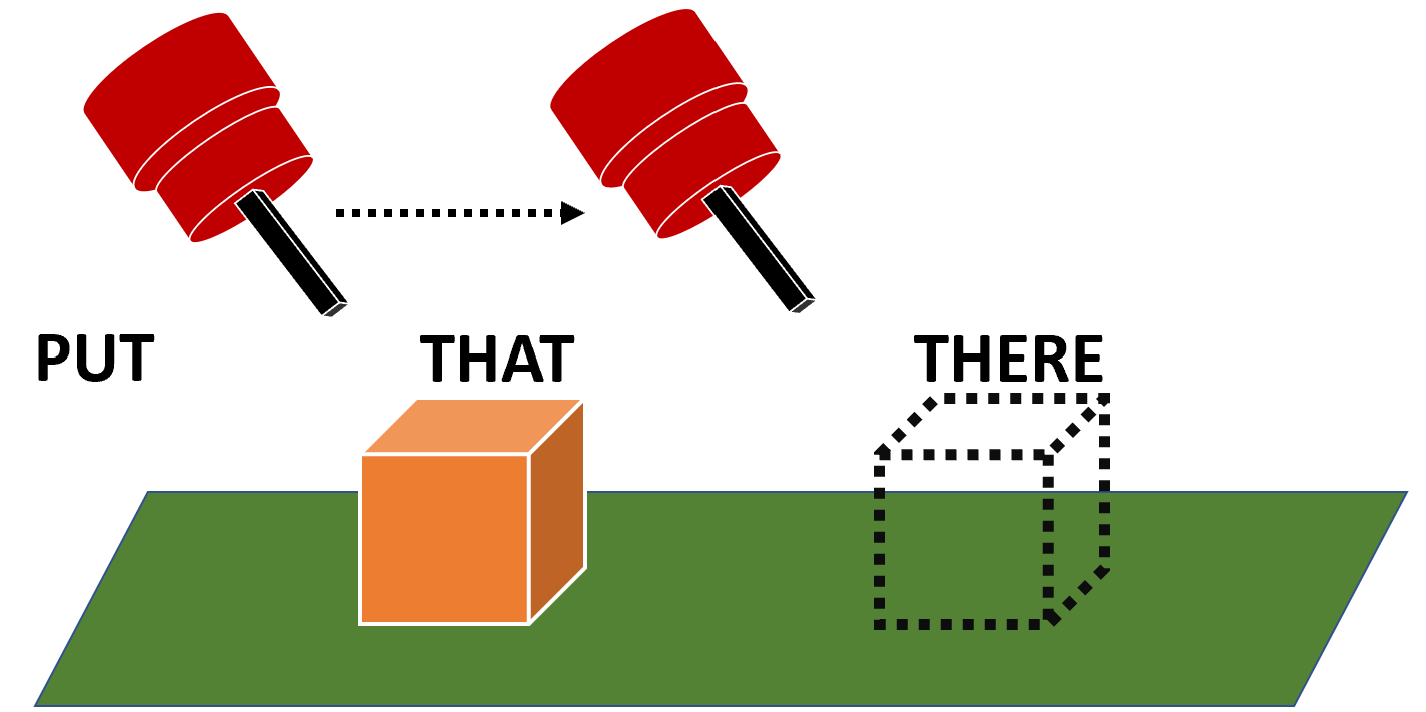
\includegraphics[width=0.45\textwidth, trim={0 0.3in 0 0in},clip]{figures/putthatthere2.png}
    \caption{A pick-and-place task requires a \textit{referential} pointing action to the object (orange cube) at the initial position, and a \textit{locating} pointing action to a final placement position (dotted cube). Such an action by a robot (in red) can also be accompanied by verbal cues like \textit{``Put that there.''}}
    \label{fig:pap}
\end{figure}

The second contribution is a set of interpretive principles, inspired by the literature on vague communication, that summarize our findings about robot pointing.  Our results suggest that pointing selects from a set of candidate interpretations determined by the type of information specified, the possibilities presented by the scene, and the options compatible with the current task.  In particular, we propose that pointing picks out all candidates that are not significantly further from the pointing ray than the closest alternatives.  Based on our empirical results, we present design principles that formalize the relevant notions of ``available alternatives'' and ``significantly further away'' and can be used in implementing future pointing robots.  The Analysis and Design Principles sections explains and justifies this approach and contextualizes it with previous research.




